\section{Project Group}

\begin{table}
\centering
\begin{tabular}{|l|c|}
\hline
Group member & Nationality \\ \hline\hline
Jon Borglund & 
\includegraphics{graphics/se} \\
Paolo Boschini & 
\includegraphics{graphics/it} \\
Kiril Goguev & 
\includegraphics{graphics/bg} \\
Faroogh Hassan & 
\includegraphics{graphics/pk} \\
Marcus Ihlar & 
\includegraphics{graphics/se} \\
Alexander Lindholm & 
\includegraphics{graphics/se} \\
Knut Lorenzen & 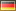
\includegraphics{graphics/de} \\
Harold Mart\'{i}nez & 
\includegraphics{graphics/ve} \\
Thomas Nordstr\"om & 
\includegraphics{graphics/se} \\
Thiago Costa Porto & 
\includegraphics{graphics/br} \\
Linus Sunde & 
\includegraphics{graphics/se} \\
Kim-Anh Tran & 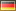
\includegraphics{graphics/de} \\
\hline
\end{tabular}
\caption{Each group member's nationality}\label{fig:nationality}
\end{table}

In our project we are 13 students coming from 7 different countries (see \fig{nationality}).
It was a great experience to have team mates from different parts of the globe - not
only working-wise but also food-wise! As our fika rule states, any person who comes later
than 9 o'clock should bring fika for the rest of the group. Thus, we could
try cheese sticks from Venezuela or Tiramisu from Italy.\\

Due the scale of the project, the group decided to divide into two teams. 
The frontend team (LISA), responsible for implementing the client side of the NetInf project and the backend team (ERNI), responsible for implementing the server technology.\\

The groups were divided as follows:

\begin{minipage}[b]{0.32\hsize}\centering
\begin{tabular}{l}
The Frontend team (LISA) \\\hline
Paolo Boschini\\
Harlold Martinez\\
Thiago Costa Porto\\
Linus Sunde\\
Kim-Anh Tran
\end{tabular}
\end{minipage}
\hfill
\begin{minipage}[b]{0.32\hsize}\centering
\begin{tabular}{l}
The Backend team (ERNI) \\\hline
Daniele Bacarella\\
Jon Borglund\\
Kiril Goguev\\
Faroogh Hassan\\
Alexander Lindholm\\
Knut Lorenzen\\
Thomas Nordstr\"om
\end{tabular}
\end{minipage}

Since we had two office rooms, each team could have one of its own.
Nevertheless, we needed to continuously communicate with each other,
since we were working on the same project with the same customer.

\subsection{Seating arrangements}
The seating arrangement of both groups are shown in \fig{frontend_seating} and
\fig {backend_seating}. The main point of the seating within both groups
was to face each other, so that social interaction and communication was facilitated. 

For bigger discussions though, the backend team used the coffee room, whereas the
frontend team had a separate discussion table in the corner of the room. Therefore
other team mates could continue working without being distracted.

\begin{figure}
\centering
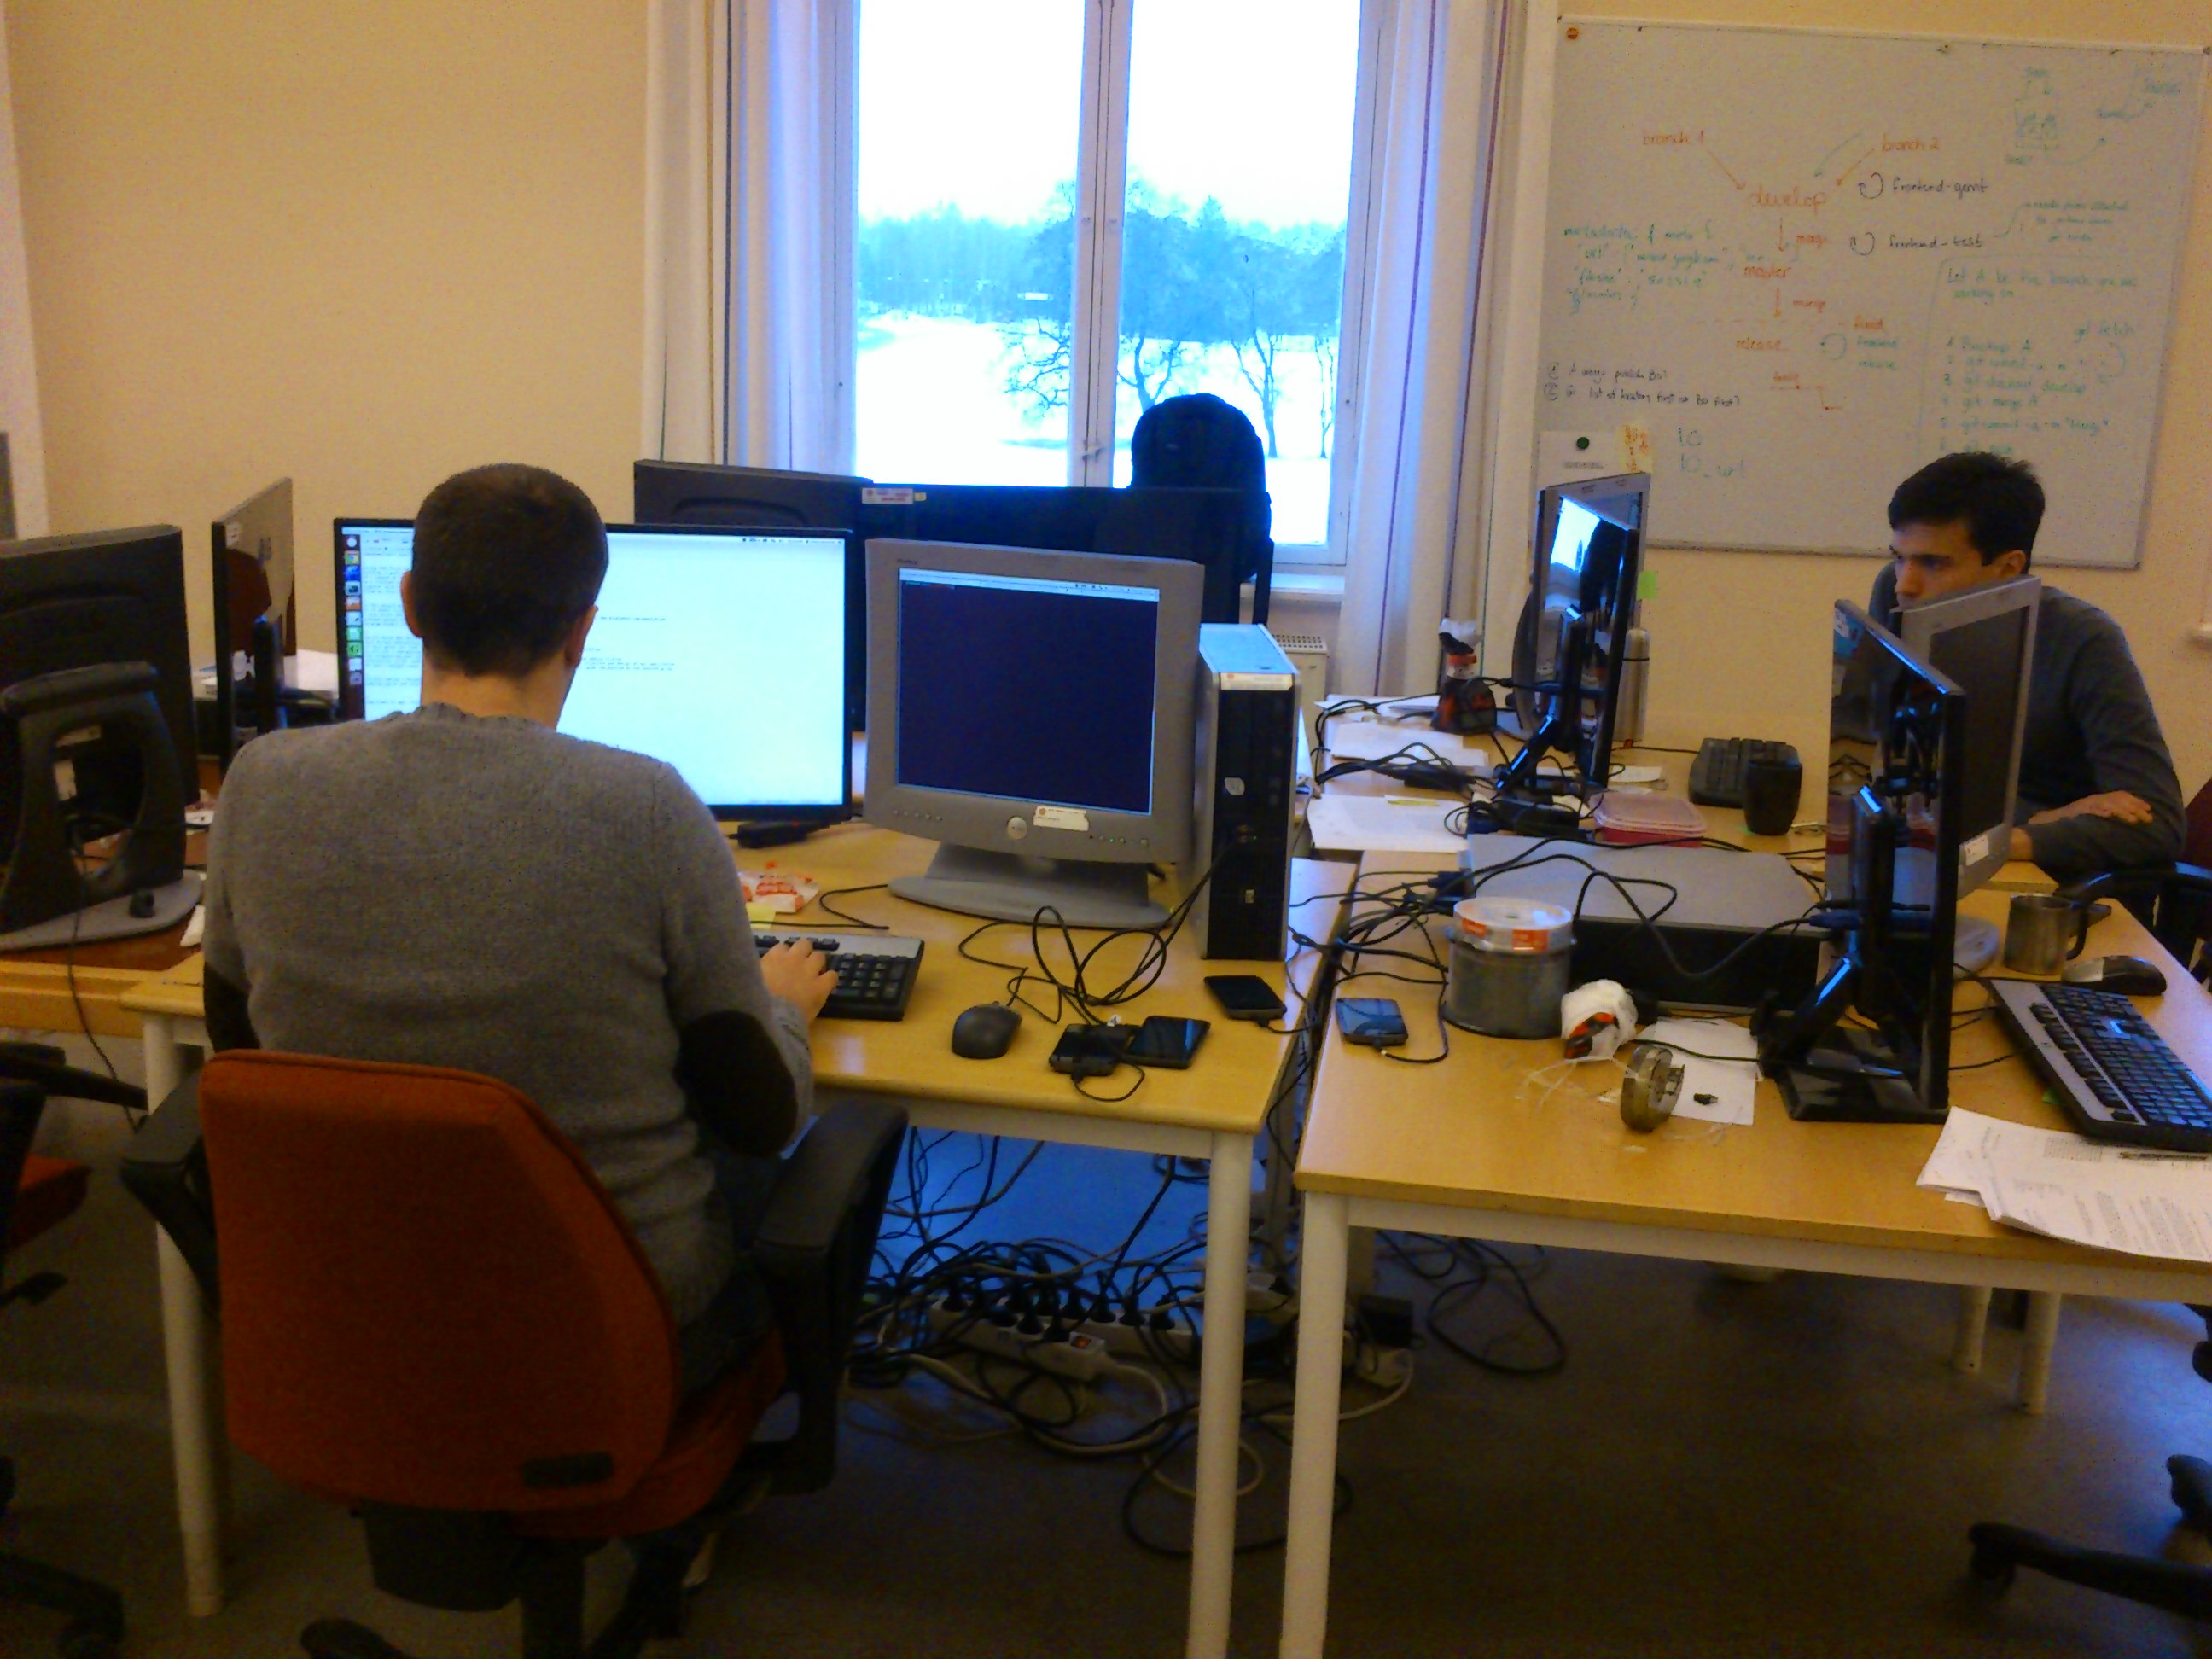
\includegraphics[scale=0.1]{graphics/frontend_seating}
\caption{Frontend seating arrangement}\label{fig:frontend_seating}
\end{figure}


\begin{figure}
\centering
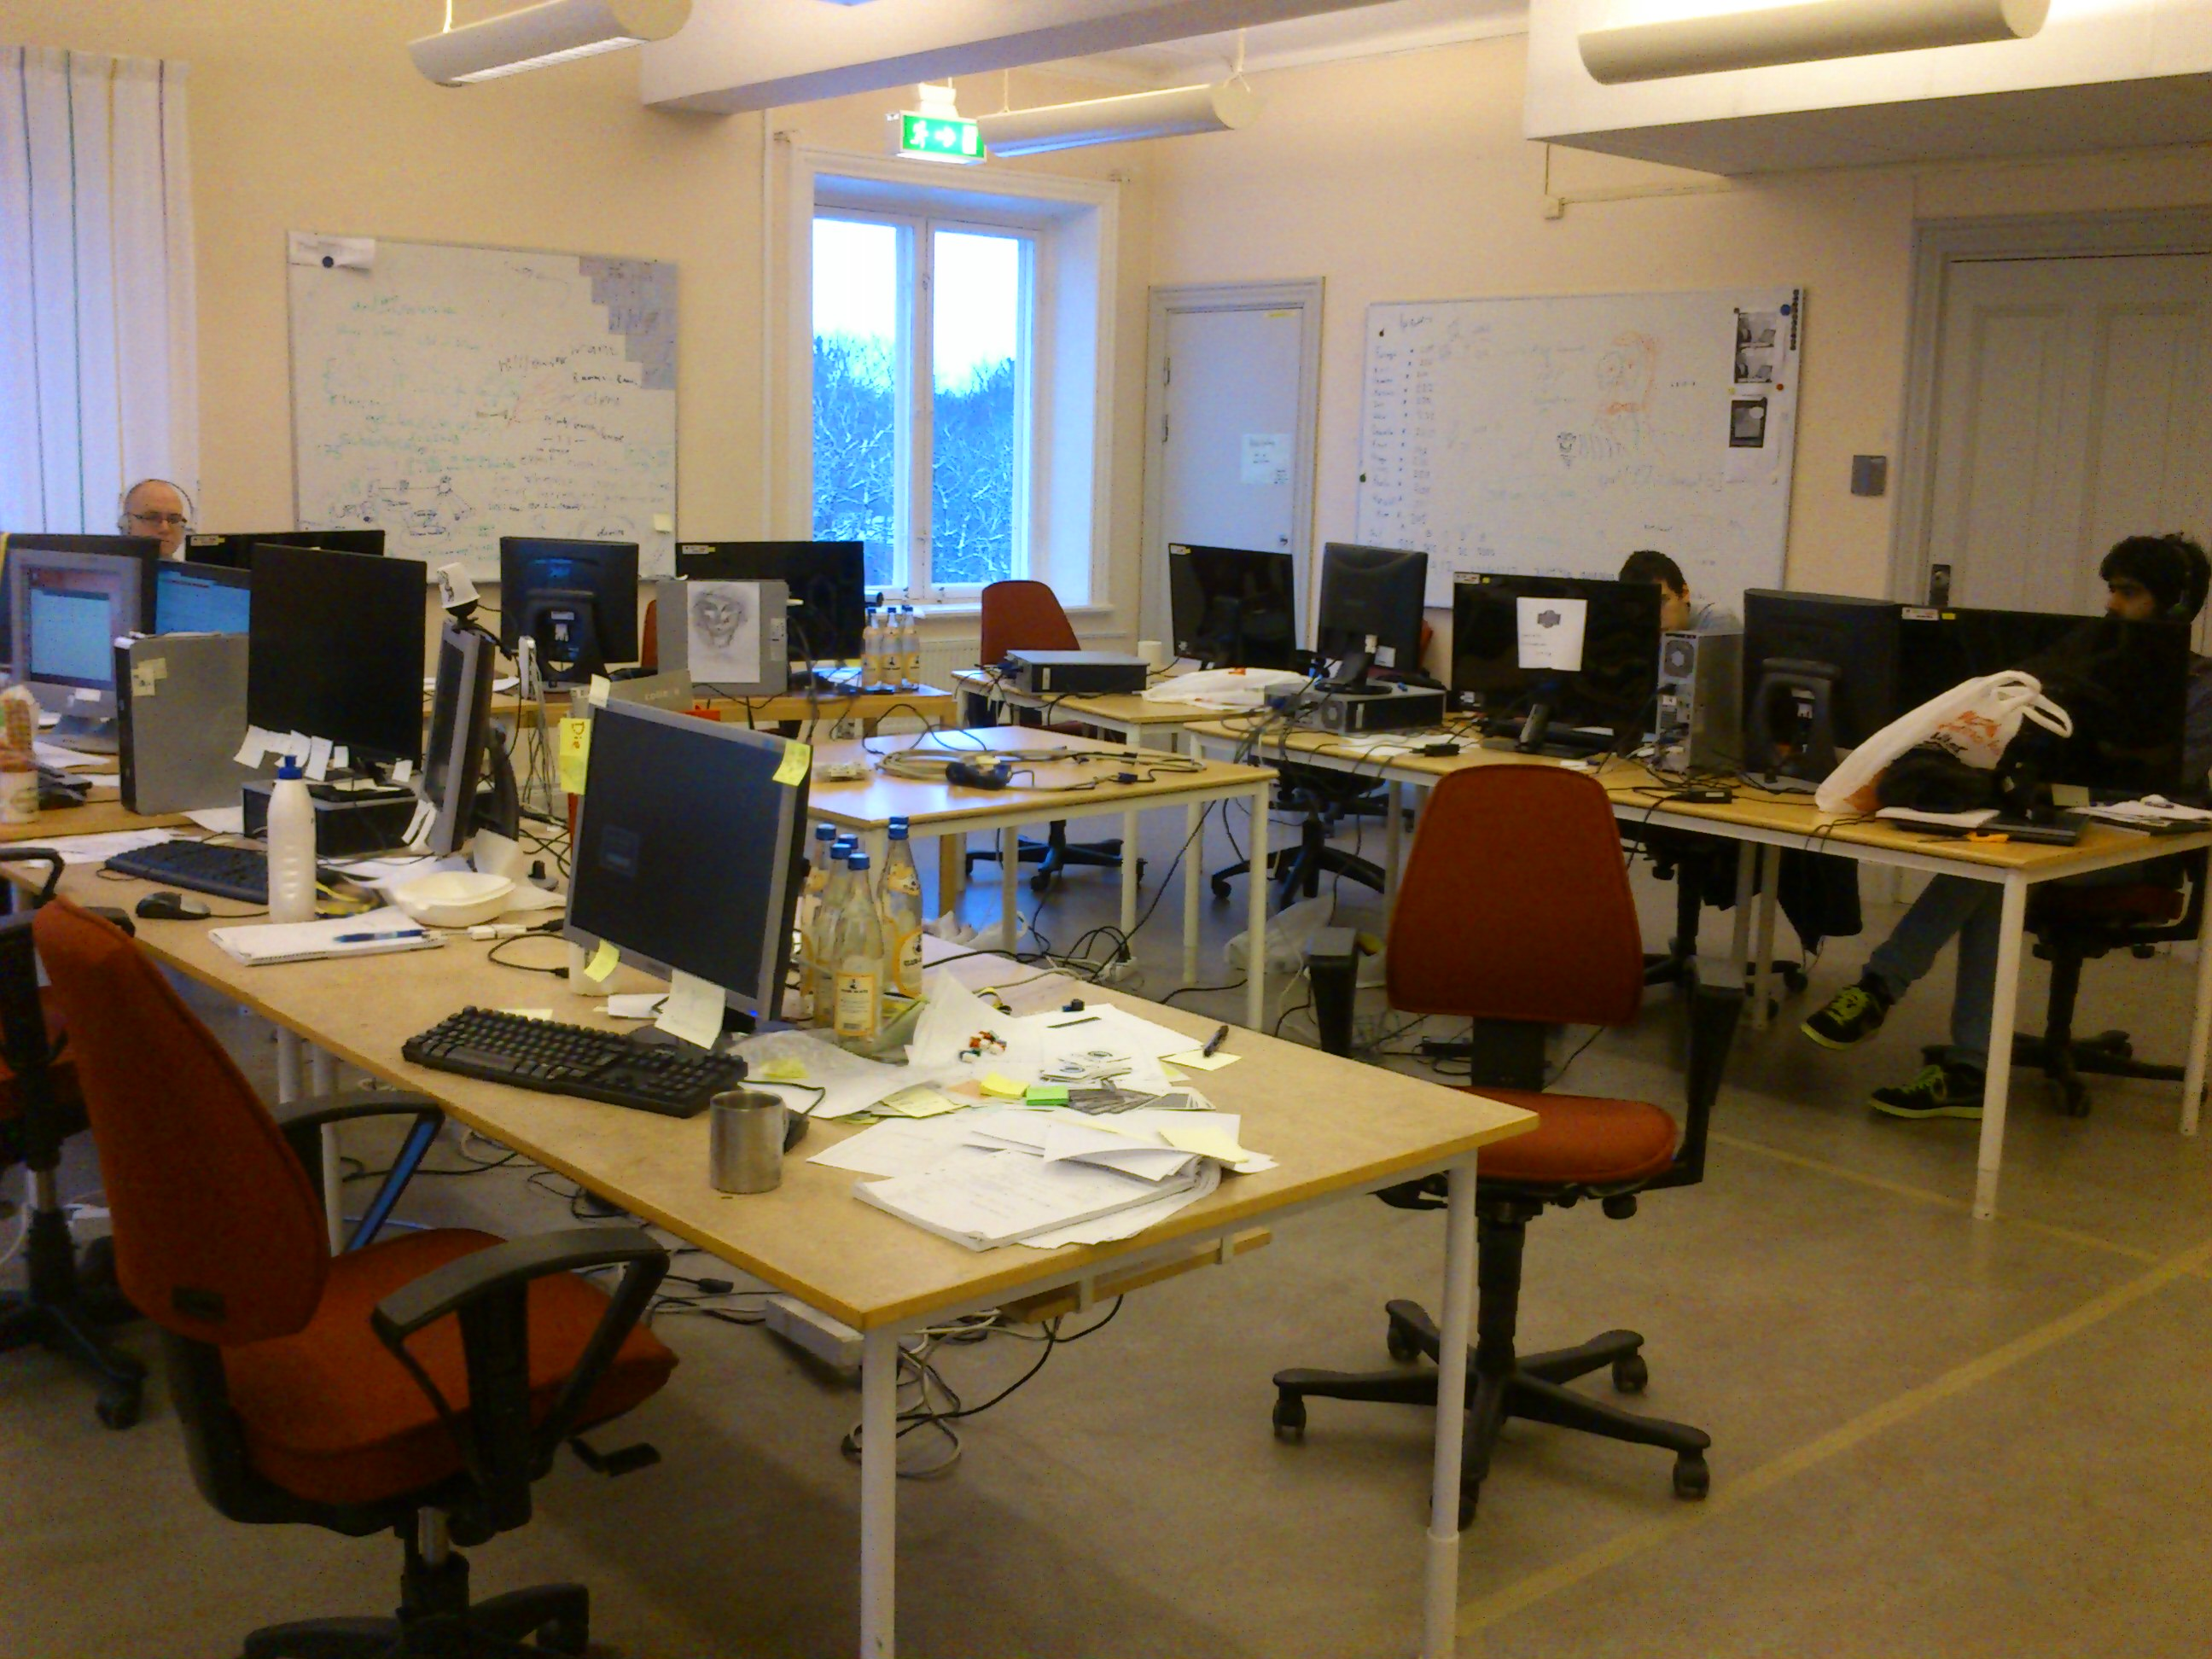
\includegraphics[scale=0.1]{graphics/backend_seating}
\caption{Backend seating arrangement}\label{fig:backend_seating}
\end{figure}
